%!TEX root = ../main.tex

\chapter{Experimente} 

\label{Experimente}

%----------------------------------------------------------------------------------------

% N O T I Z E N
% Cartoonset, MNIST, (WIND)
% PCA, UMAP, t-SNE, LargeVis

% random repulsive forces?

% neg. sampling = 0

% eigenvalues in Alg4

% keine Optimierung

% Strategie zum finden der Parameter (notwendig?)

% T E X T B A U S T E I N E
% 'Empirisches testen der Hypothesen/ Annahmen'
% 'UMAP auf realen/echten Daten'
% In \cite{UMAP} wurde bereits die Stabilit�t des Verfahrens getestet.
% Insbesondere verweisen wir auf Abbildung 3,4 in Abschnitt 5.
% Die Stabilit�t des UMAP Verfahrens ist 
%----------------------------------------------------------------------------------------
%----------------------------------------------------------------------------------------
Nach ausf�hrlicher Darstellung der Theorie des UMAP Verfahrens, m�chten wir nun UMAP auf 
zwei Datens�tzen mit alternativen Verfahren vergleichen.
Wir werden eine m�glichst vollst�ndige Darstellung der Ergebnisse in dieser Arbeit pr�sentieren. 
Allerdings ist es zu empfehlen die Ergebnisse in einem interaktiven Jupyter notebook zu betrachten. 
Dieses befindet sich auf der beigelegten CD. %TODO: CD und/oder Link?

\section{Alternative Verfahren}
% TODO: Liste mit t-SNE, Fit-SNE, PCA, ISOMAP, LargeVis. 
% Kurz was macht das verfahren aus; Link; wichtige Hyperparameter
Wir haben uns dazu entschieden UMAP mit folgenden Verfahren zu vergleichen:

\subsection*{t-SNE}
Das t-SNE Verfahren \cite{tSNE} ist zur Zeit eines der bekanntesten und meistgenutzten 
nicht linearen Dimensionsreduktionsverfahren. 



\section{Cartoon Set}
In diesem Abschnitt werden wir den \textit{Cartoon Set} Datensatz analysieren \cite{cartoon}. 
Dabei werden wir:
\begin{itemize}
	\item sehen, dass UMAP eine vergleichbare Laufzeit mit der von FIT-SNE hat
	\item das Verhalten der niedrigdimensionalen Darstellung unter verschiedenen 
		  Hyperparametern betrachten
	\item eine exemplarische Beschreibung der Hyperparameter geben
	\item UMAP mit anderen Dimensionsreduktionsverfahren vergleichen
	\item sehen, dass UMAP zugrundeliegende Mannigfaltigkeiten erkennt und darstellt
\end{itemize}

%-----------------------------------

\subsection{Beschreibung des Datensatzes}
Der Cartoon Datensatz enth�lt \num{100000} unterschiedliche Bilder von gezeichneten Gesichtern 
(siehe \ref{fig:Cartoon_Sample}). 

\begin{figure}
	%\centering
	
\includegraphics[width=400px, height=73px]{Figures/Cartoon_Sample}
	%\decoRule
	\caption[Ausschnitt des Cartoon Set]{Sechs zuf�llig gew�hlte Gesichter des Cartoon Set.}
	\label{fig:Cartoon_Sample}
\end{figure}

Die Bilder wurden aus 16 Komponenten zusammengesetzt (u.a. Gesichtsform, Gesichtsfarbe, Frisur, Haarfarbe), 
dabei variiert die Anzahl der M�glichkeiten pro Komponente zwischen zwei (Augenlied, Wimpern,\dots) und 
111 (Anzahl m�gliche Frisuren). 
Die Farben der Komponenten wurden aus einem diskreten RGB Raum gew�hlt. Insgesamt ergibt sich eine m�gliche 
Anzahl von $10^13$ Gesichtern.

F�r die Analyse haben wir verschiedene Eigenschaften zusammengefasst um einen besseren �berblick zu haben. 
Beispielsweise haben wir die 111 Frisuren, nach qualitativer Analyse, zu 19 Frisurtypen zusammengefasst. 

Wir haben uns f�r diesen Datensatz entschieden um UMAP auf Daten mit einer komplexeren Struktur zu testen 
als dies in \cite{UMAP} gemacht wird. Dabei ist auch zu beachten, dass es aufgrund der 16 Komponenten aus 
welchen die Gesichter bestehen kein richtige oder falsche Einbettung der Daten gibt. 

Wir haben die Bewertung der Einbettung unter der Annahme gemacht, dass \textit{�hnliche} Gesichter 
\textit{�hnliche} Hautfarben, Frisuren, Haarfarben, Brillen und B�rte haben. Diese f�nf Eigenschaften 
m�chten wir besonders hervorheben, da sie die dominantesten Merkmale des Gesichts beschreiben.

Die urspr�ngliche Gr��e eines Bildes betrug $500 \times 500$ Pixel mit vier Farbkan�len 
(CYMK-Darstellung der Farben). Aufgrund des gro�en Randes haben wir uns dazu entschieden die Gr��e der 
Bilder auf $300 \times 300$ ohne nennenswerten Informationsverlust zu verringern. Weiterhin haben wir uns 
f�r die Bewertung der Einbettung auf \num{10000} Bilder beschr�nkt. % TODO: Bewertung f�r 100000 samples?
Somit betr�gt die Dimension 
des Cartoon Set $D = \num{360000}$ und die Anzahl an Beispielen $N = \num{100000}$.



\section{Laufzeitanalyse}
Die praktischen Tests der Verfahren wurden auf Rechnern mit einer Linux-Architektur ausgef�hrt. 
Die CPU Tests haben wir auf Intel Xeon 6136 CPUs mit 48 Kernen und 384 GB RAM ausgef�hrt. 
F�r die Verfahren welche mittels Berechnungen auf einer Graphikkarte verbessert wurden, haben 
wir Intel Xeon Gold 6136 CPUs mit 188 GB RAM und Nvidia V100 GPUs genutzt. 
Insgesamt haben wir �ber 100 Experimente gemacht um genauere Aussagen �ber die Laufzeit der Verfahren 
zu treffen und diese in Abh�ngigkeit der wichtigen Parameter zu setzen.


\begin{figure}
	%\centering
	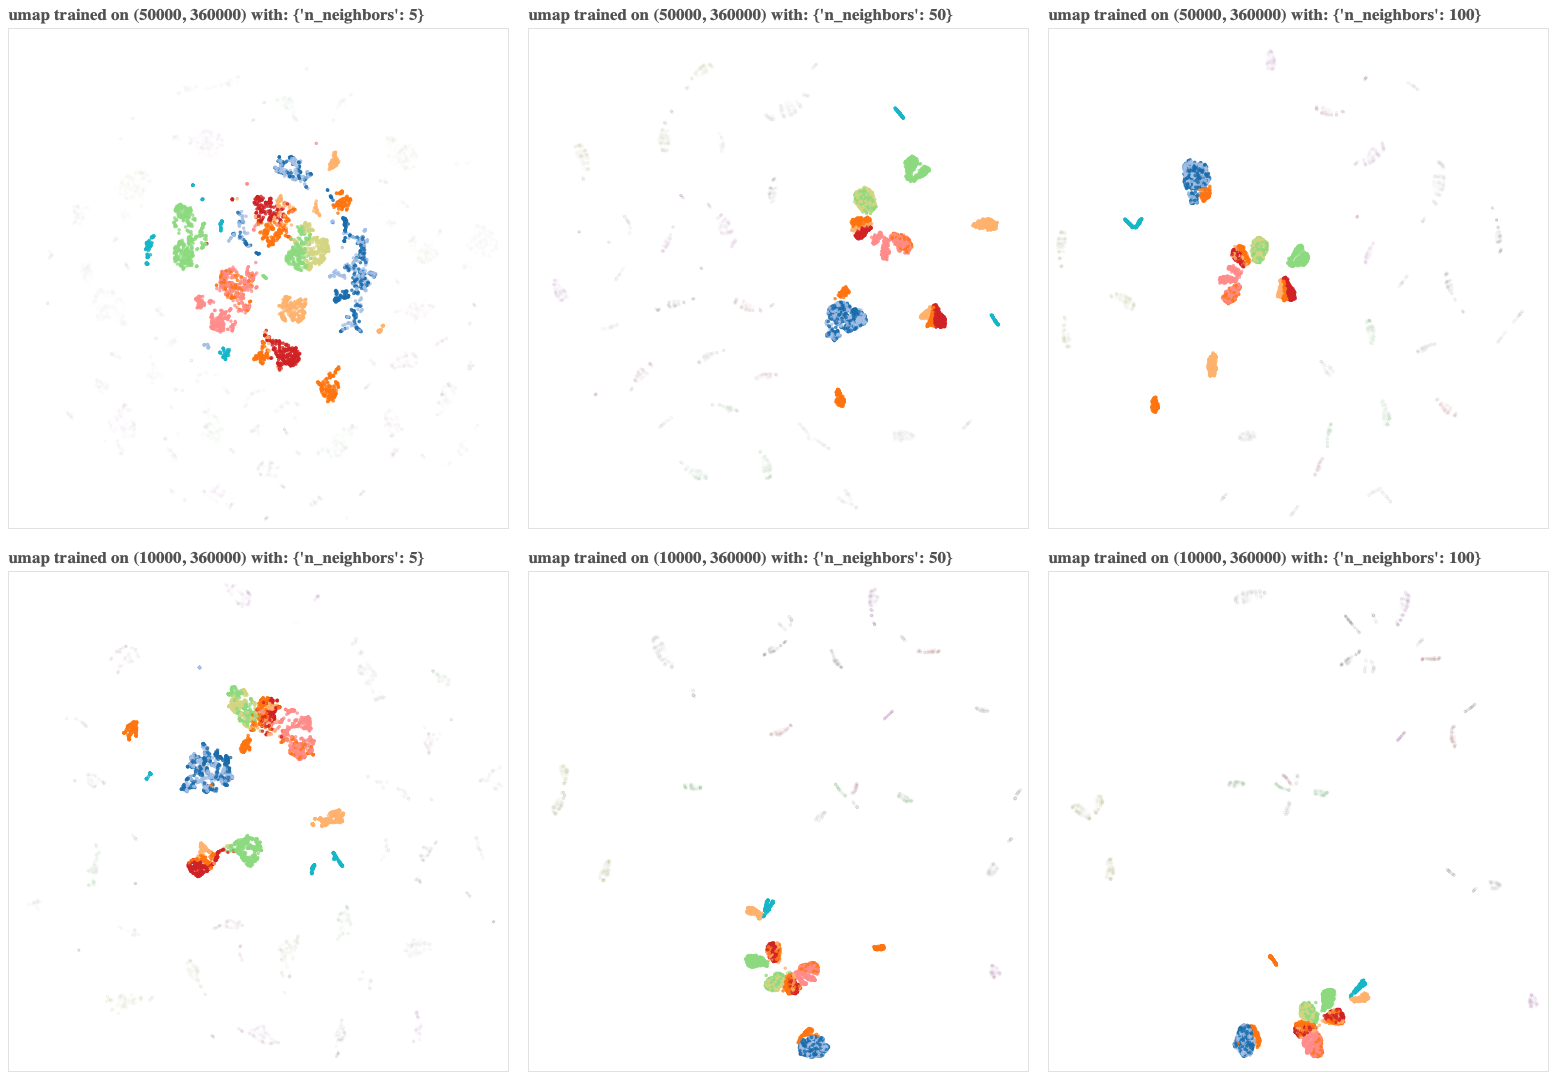
\includegraphics[width=400px, height=278px]{Figures/umap_10k_vs_50k}
	%\decoRule
	\caption[UMAP auf 50k und 10k Daten]{TODO: Beschreibung des Bildes}
	\label{fig:umap_10k_vs_50k}
\end{figure}






